\begin{sagesilent}
iimport matplotlib.pyplot as plt
import numpy as np

d = load("sobj/oscilloscopio-c2.sobj", verbose=False)

plt.clf()
plt.ylim(ymin=3, ymax=15)
plt.title("Grafico 1")
plt.xlabel("Frequenza (Hz)")
plt.ylabel("Corrente (mA)")
plt.grid(True, which='both')
plt.loglog(d['frequenza_hz'], d['i_ma'], '.r')
plt.savefig("grafici/C2-1.png")

plt.clf()
plt.ylim(ymin=0.3, ymax=1.5)
plt.grid(True, which='both')
plt.loglog(d['frequenza_hz'], d['valore_mu']/d['v_rms'], '.r')
plt.savefig("grafici/C2-2.png")
\end{sagesilent}


\chapter{Misura della velocità della luce}

L'obiettivo del nostro esperimento è misurare la velocità della luce $c$.

L'apparato di misurazione consiste principalmente in:
\begin{itemize}
 \item Un laser Elio-Neon ($\lambda=632$ nm).
 \item Uno specchio rotante a velocità angolare regolabile.
 \item Due lenti convergenti, di lunghezza focale $l_1 = 48$mm e $l_2 = \sage{f}$mm.
 \item Un microscopio con beam splitter e micrometro.
\end{itemize}

Durante l'esperimento viene puntato un laser su di uno specchio rotante, fatto rimbalzare su di uno specchio fisso, e dopo un'altra riflessione sullo specchio rotante raccolto e misurato tramite un microscopio.

Lo specchio rotante viene fatto girare con velocità angolare $\omega_1$ in senso orario e $\omega_2$ in senso antiorario. Queste velocità angolari sono (in modulo) identiche nella maggior parte dei casi, o con differenza trascurabile, dunque da qui in avanti si parlerà semplicemente di velocità angolare $\omega$.

Si misura a questo punto lo spostamento del punto luminoso visualizzato nel microscopio, tramite cursori e micrometro. A seconda della velocità angolare dello specchio rotante si osserverà uno spostamento del puntino nel microscopio, dovuta alla rotazione dello specchio durante il tempo di volo dei fotoni. Ci aspettiamo che questa dipendenza tra spostamento e velocità angolare sia di tipo lineare.

Chiamando $s_{cw}$ e $s_{ccw}$ rispettivamente le misure con specchio rotante in senso orario e antiorario, per come è orientata la strumentazione il numero
$$\Delta s = s_{cw} - s_{ccw}$$
deve essere positivo.

Purtroppo però non è questo il caso per qualche misura presa in mattinata, per ragioni sconosciute e che non siamo riusciti a riprodurre. Questi dati sono esclusi dall'analisi in quanto evidenti errori, e sono mostrati in rosso nel grafico seguente.

/*I dati sono molti, dunque forniamo qui soltanto una visione grafica, e lasciamo la tabella come allegato alla fine della relazione.*/

\section{Analisi dati}

Chiamiamo $D = \sage{d}$mm la distanza specchio rotante/specchio fisso, $A$ la distanza del punto di convergenza del fascio laser dalla lente $l_2$ e $B$ la distanza tra $l_2$ e lo specchio rotante. Misuriamo $B$ e $D$ con l'aiuto di un metro a nastro.

Per calcolare con precisione $A$, conoscendo la distanza focale di $l_2$, la ricaviamo dalla formula dei punti coniugati:
$$A=\frac{(B+D)f}{B+D-f} = \sage{n(a, digits=4)} \text{mm}$$


Per calcolare $c$, dobbiamo interpolare linearmente:
$$\Delta s = \frac{\tilde{A}}{c}\omega\qquad (= m\omega)$$
ove
$$\tilde{A} = 4\frac{AD^2}{D+B}$$
ricavata dalla geometria del problema.

\begin{sagesilent}
var('m, q')
model(x) = m*x+q
dataprime = [(sp[i], diff[i]) for i in range(0, len(sp))]
fit = find_fit(dataprime, model, solution_dict = True)
model2(x) = m*x
fit2 = find_fit(dataprime, model2, solution_dict = True)

at = 4*a*d^2/(d+b)
plot_experiment(fit[m], fit[q]) 
\end{sagesilent}

L'interpolazione viene fatta sulla funzione
$$y=mx+q$$
in cui abbiamo lasciato libero il parametro $q$.

Risulta coerente la stima di fit $q=\sage{n(fit[q], digits=2)}$, compatibile con il valore 0 visti i valori e le grandi incertezze sperimentali, difficilmente stimabili a priori.

La funzione che ci permetterà di calcolare $c$ è ora banale, e con in nostri dati vale:

$$c = 2\frac{\tilde{A}}{m} = \sage{n(2*at/fit[m], digits=4)} \text{m/s}$$

Abbiamo anche provato a imporre il passaggio per l'origine ($q = 0$), nel qual caso
$$c = 2\frac{\tilde{A}}{m} = \sage{n(2*at/fit2[m], digits=4)} \text{m/s}$$

Il fattore 2 è introdotto in quanto la differenza non viene misurata tra specchio fermo e specchio rotante, ma con specchio rotante nelle direzioni opposte.

\begin{center}
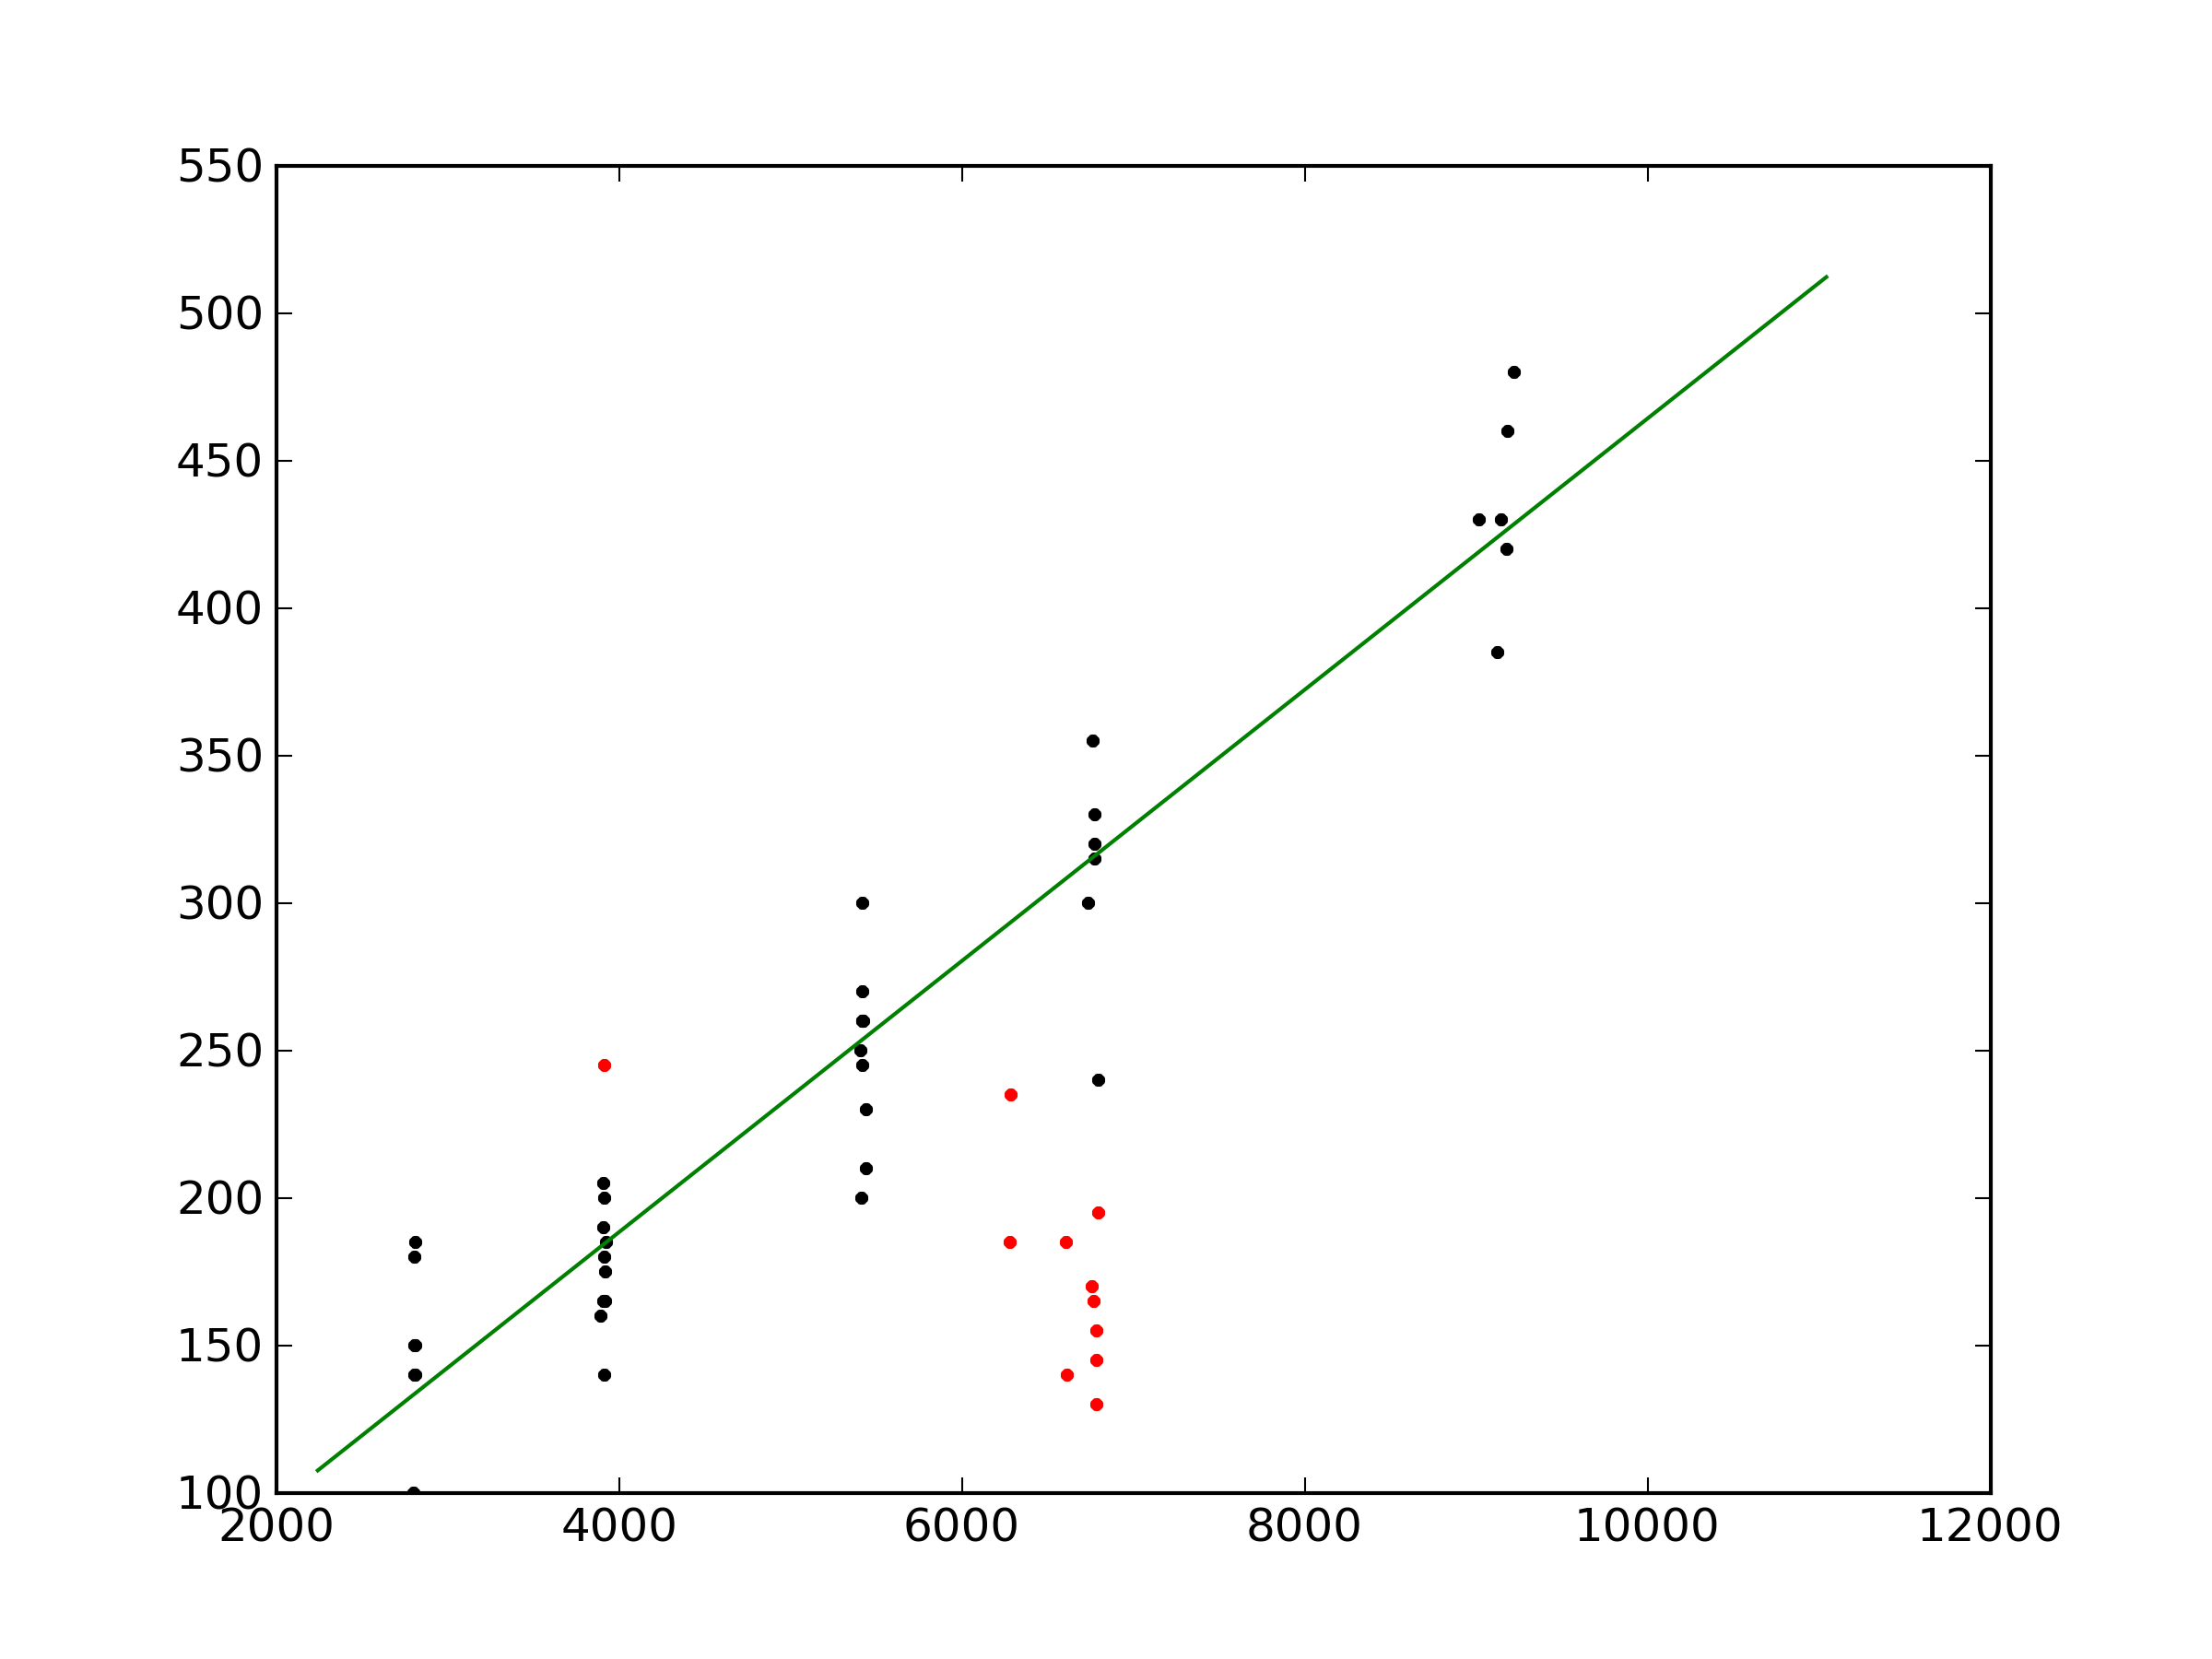
\includegraphics[scale=0.75]{grafici/C/dati.png}
\end{center}

Valutiamo la bontà del nostro fit con il test del $\chi^2$. L'errore è evidentemente maggiore dell'errore dovuto alla precisione strumentale (5 $\mu$m), e dunque utilizzeremo la stima a posteriori degli errori. Con questi dati otteniamo:

\begin{sagesilent}
# Chi quadro
def funct(x):
    return fit[m]*x+fit[q]

chi = 0
for i in range(0,len(diff)):
    teo = model.subs(x=sp[i], m=fit[m], q=fit[q])
    chi += (diff[i]-teo)^2/teo
    
chinoq = 0
for i in range(0,len(diff)):
    teo = model2.subs(x=sp[i], m=fit2[m])
    chinoq += (diff[i]-teo)^2/teo
    
chirid = chi/(len(diff)-3)
chiridnoq = chinoq/(len(diff)-2)
\end{sagesilent}

$$\chi^2 = \sage{n(chi, digits=4)}$$
$$\tilde{\chi}^2 = \sage{n(chirid, digits=4)}$$
Per quanto riguarda il fit senza $q$
$$\chi^2 = \sage{n(chinoq, digits=4)}$$
$$\tilde{\chi}^2 = \sage{n(chiridnoq, digits=4)}$$

\section{Allegato: dati}
\begin{sagesilent}
def stampa_dati(vel, deltas, col1, col2):
  s = r"\begin{tabular}{c|c}"
  s += "%s & %s \\\\" % (col1, col2)
  s += r"\midrule"
  for i in range(0, len(vel)):
    s += "%d & %d \\\\" % (vel[i], deltas[i])
  s += r"\end{tabular}"
  return s
\end{sagesilent}

\begin{center}
 \sagestr{stampa_dati(sp, diff, r"$\omega$ ($rad/s$)", r"$|\Delta s|$ ($\mu$m) ($\pm5\mu m$)")}
\end{center}
Dati scartati:
\begin{center}
 \sagestr{stampa_dati(sp2, diff2, r"$\omega$ ($rad/s$)", r"$|\Delta s|$ ($\mu$m) ($\pm5\mu m$)")}
\end{center}
